% Set the author and title of the compiled pdf
\hypersetup{
	pdftitle = {\Title},
	pdfauthor = {\Author}
}

\section{Introduction}

We want computers to be able to interact with us, just like we interact with
them. This involves having them understand written text and voiced speech, as
well as being able to synthesise speech and text themselves. This includes
things like translation text and searching for key words in text.

A computer or a suite of programs that can do all of this is the goal for
Natural Language Systems. The catch is, that language is hard and complicated,
and to make computers do the things we want them to, we need to know how3
language works, and express this as an executable program.

Language is the representation of ideas, and the linkage of different ideas
together in such a way as to create new ideas. In order to understand any one
sentence (a sentence usually corresponds to one idea, event or action), we have
to understand what each symbol in the language means in isolation, and
understand how they're connected, and what the connections to do change the
meaning of the ideas.

Many factors affect the meaning of a sentence, but the connection between words
is always hierarchical, and we can represent sentences as trees:

\begin{figure}[ht]
  \centering
  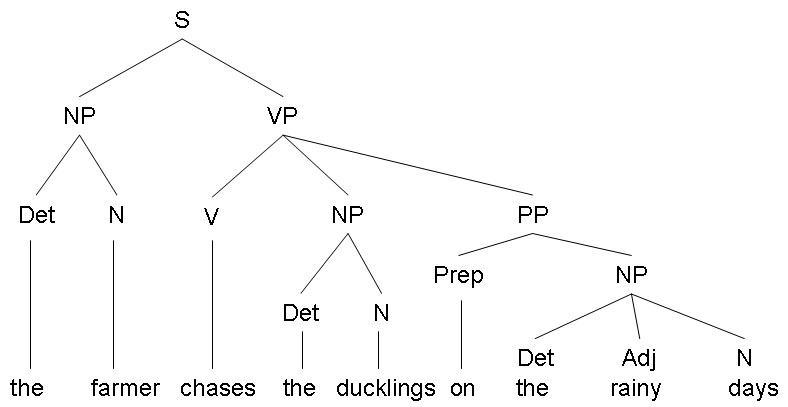
\includegraphics[width=0.55\textwidth]{images/phase-structure-tree}
  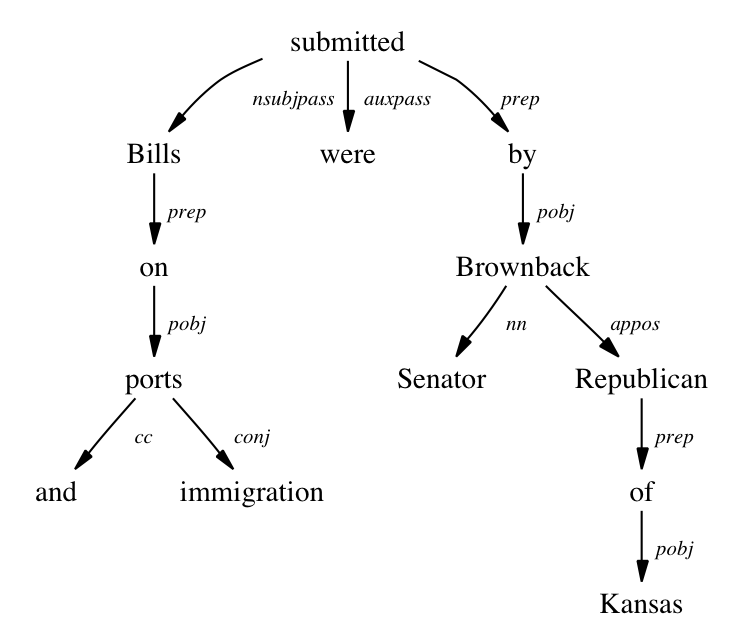
\includegraphics[width=0.35\textwidth]{images/dependency-tree}
  \caption{The left image is a phase structure tree, and the right image is a
  dependency tree.}
  \label{fig:trees}
\end{figure}

A parse tree is all well and good, but to a computer, this is only slightly more
useful than the original text. Though we have extracted some information out of
the text, we still just have a hierarchy of words, but we want a hierarchy of
ideas.

Having ideas instead of words allows us to infer more than what the text
literally says:

\begin{itemize}
  \item I'm fixing my motorbike $\rightarrow$ This person possesses a
  motorbike, and it is currently broken.
  \item The cake smells good $\rightarrow$ There is cake somewhere. Somebody is
  close enough to smell it.
\end{itemize}

But how can we do that?

\section{Structural analysis}

It is possibly to try and find out the meaning of a word simply by looking at
what letters it is made up of. One way to do this is to split a word into
\textbf{morphemes}, which are the most basic meaning-carrying components of a
word, and try to associate a meaning with each. For example \textit{undone}
could be split into \textit{un} and \textit{done}, and meaning associated with
each.

\subsection{Tries}

\marginpar{Tries are very handy datastructures for technical interviews, you
should read up on them an implement one!}

In order to examine the syntactic and semantic properties of the words, we need to represent them in the computer. A common way to do this is with a \textit{trie}:

\begin{wrapfigure}{r}{0.25\textwidth}
  \begin{center}
    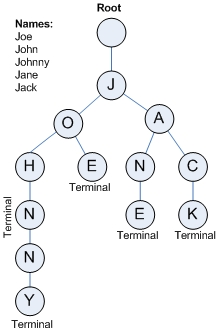
\includegraphics[width=0.24\textwidth,keepaspectratio]{images/trie}
  \end{center}
  \caption{A trie storing some names.}
\end{wrapfigure}

Tries are very memory efficient, since they if multiple words share the same
prefix, then the prefix is only stored once in memory. Tries have a lookup time
of $O(m)$, where $m$ is the length of the word, which is quite good, and is
better than a hash table in terms of speed in some cases. If you're stupid
enough to represent your dictionary as a list of words, then you can do a binary
search if its ordered (worst case $O(log(n) * m)$ comparisons (the $m$ comes
from having to possibly compare each character in the word)), or a linear search
if it isn't ordered ($O(m*n)$ in the worst case!).

\subsection{Spelling rules}

We want to understand why combining \textit{big} and \textit{est} produces
\textit{biggest} with an extra \textit{g}. Why isn't it \textit{bigest}? The
reason why we want to understand this, is so we can go from a word that we're
processing in text, and pick it apart into its components so we can better
understand it.

That is to say, we're going from \textit{biggest} to \textit{big} +
\textit{est}.

The format of the rules we're using in the course is as follows:

\marginpar{You can use \texttt{cX} and \texttt{vX} where \texttt{X} is an
integer, and \texttt{c/v} denotes a consonant or vowel inside the context
brackets.}

\begin{verbatim}
  [from] ==> [to]: [prevContext] _ [nextContext];
\end{verbatim}

For example, if we had a rule like:

\begin{verbatim}
  [g] ==> []: [g] _ [e,s,t];
\end{verbatim}

It would turn \textit{biggest} into \textit{big} + \textit{est}.

\subsection{Categorical descriptions}

Even if we find the meaning of every word by splitting it info morphemes, we
just end up with a collection of words that we know the construction of, but
we're still no closer to understanding a sentence.

In order to find the relationships between words in a sentence, we should use
the approach in Figure~\ref{fig:trees}, and try to fit the words into some tree
structure.

One way of doing this, is to specify lots of different forms that a sentence can
take. For example `noun verb noun' might describe a sentence such as `Todd
writes notes'. Providing that we have some \textit{prototype} for a sentence
that fits the words that we've been given, we can ascertain that we can in fact
make a sentence out of these words.

There is a better approach though. Each word in a sentence changes its meaning
in some way, and we can put words into buckets according to how the meaning of
the sentence is changed; for example, a verb specifies what kind of event is
happening. Having a verb on its own doesn't do us much good; we will know that
\textit{something} is happening, but not where, why, what, when etc. Verbs need
other parts of sentence around them to make them work.

We can treat each word as part of a jigsaw, specifying what other words or
phrases it needs in order to have meaning, and then fit the pieces together
according to some schema.

We need to specify a schema with which we can specify what different words require:

\begin{verbatim}
  <word> = <rules>
\end{verbatim}

The rules are their own language, which has a few rules. Brackets are
treated as they usually are in maths, and the only other special characters are
forward and backward slashes. These indicate whether a word or phrase should be
before or after the word.

\begin{verbatim}
  writes = (s\np)/np
\end{verbatim}

This indicates that the word `writes' needs a noun phrase (\texttt{np}) to its
right and then a noun phrase to its left to make a sentence (\texttt{s}).

With the right set of rules for each word, we can now parse sentences:

\begin{verbatim}
  writes = (s\np)/np
  Todd = np
  notes = np
\end{verbatim}

\begin{center}
  % Tabular centering hack
  \begin{tabular}{c}
    \begin{lstlisting}
      Todd        writes        notes
       np       (s\np)/np        np
                ---------------------
                        s\np
      -----------------------
                s
    \end{lstlisting}
  \end{tabular}
\end{center}

Here, the words `Todd' and `notes' are \textit{saturated} since they don't
require anything else to make them into complete `items'. `writes' is
unsaturated, since it needs other stuff to make it into a complete item. Word
rules of these kind are called \textbf{Categorical Descriptions}.

\subsection{Morphology}

Now we've figured out how to decompose a word into morphemes using spelling
rules, and we can fit these words into a sentence. However, we also want to know the precise meaning for each word (this helps when arranging them in a sentence too). We can do this by looking at each morpheme.

There are two types of morphology that we're going to look at:

\begin{description}
  \item \textbf{Inflectional morphology}\\
    This is when the stem of the word is incomplete, and other morphemes 
    provide more information to specify exactly what we mean:

    \begin{itemize}
      \item `sing' + `ing' = verb + present participle
      \item `work' + `ed' = verb + past participle
      \item `work' + `' = noun + singular
    \end{itemize}

  \item \textbf{Derivational morphology}\\
    This is where the meaning of the stem is significantly changed by other 
    morphemes. For example, `smelly' could be combined with `er' to give 
    `smellier', or `est' to give `smelliest'. Obviously we need spelling rules 
    to do this correctly!
\end{description}

We need a way to specify what words can have what suffixes/affixes. For example,
`conscript' can be combined with `tion' to give `conscription', but not `ly' to
give `conscriptly'.

Furthermore, there are spelling rules concerned with adding bits onto words; as
we saw before, `smelly' becomes `smellier', not `smellyer'. We will come across
this later though.

It turns out that composing morphemes is similar to composing words. We can use the same notation:

\begin{verbatim}
  'conscript' = noun>agr
  'conscript' = verb>tns
  'tion' = (noun>agr)<(verb>tns)
  'ing' = tns
  'ed' = tns
  's' = agr
  '' = agr
\end{verbatim}

These descriptions allow you to construct the following words:

\begin{mymulticols}
  \begin{itemize}
    \item conscript (noun)
    \item conscripts (noun)
    \item conscription (noun)
    \item conscriptions (noun)
    \item conscripting (verb)
    \item conscripted (verb)
  \end{itemize}
\end{mymulticols}

However, the rules are not perfect, and will also allow you to make:

\begin{mymulticols}
  \begin{itemize}
    \item conscriptingtion (noun)
    \item conscriptedtion (noun)
    \item conscriptingtions (noun)
    \item conscriptedtions (noun)
  \end{itemize}
\end{mymulticols}

We can also make rules cancel out. If we have a rule that is `verb$>$tns' and
another that is `tns$>$agr' then we can make a `verb$>$agr' from them.

To see a worked example of these rules, and how they're applied, look on slides
$64-110$ in the
\href{http://studentnet.cs.manchester.ac.uk/ugt/2015/COMP34411/COMP34411.pdf}
{course notes}.

One thing that is important to note, is that we can process words from left to
right, and don't have to back-track. This means that processing is in linear
time, which is fantastic (though we need a big dictionary of words, which is
rather less fantastic).
